\documentclass[12pt]{amsart}
\usepackage[margin=1in]{geometry}
%\geometry{letterpaper}                   % ... or a4paper or a5paper or ... 
%\geometry{landscape}                % Activate for for rotated page geometry
%\usepackage[parfill]{parskip}    % Activate to begin paragraphs with an empty line rather than an indent
\usepackage{graphicx}
\usepackage{amssymb}
\usepackage{epstopdf}
\usepackage{hyperref}
\usepackage{listings}
\usepackage{multirow}
\usepackage{lipsum}
\usepackage{enumerate}
\usepackage{setspace}
\usepackage{color}
\pagenumbering{gobble}

\definecolor{lightgray}{rgb}{.9,.9,.9}
\definecolor{darkgray}{rgb}{.4,.4,.4}
\definecolor{purple}{rgb}{0.65, 0.12, 0.82}
\lstdefinelanguage{JavaScript}{
  keywords={break, case, catch, continue, debugger, default, delete, do, else, false, finally, for, function, if, in, instanceof, new, null, return, switch, this, throw, true, try, typeof, var, void, while, with},
  morecomment=[l]{//},
  morecomment=[s]{/*}{*/},
  morestring=[b]',
  morestring=[b]",
  ndkeywords={class, export, boolean, throw, implements, import, this},
  keywordstyle=\color{blue}\bfseries,
  ndkeywordstyle=\color{darkgray}\bfseries,
  identifierstyle=\color{black},
  commentstyle=\color{purple}\ttfamily,
  stringstyle=\color{red}\ttfamily,
  sensitive=true
}

\lstnewenvironment{mylisting}
  {\singlespacing \lstset{
   language=JavaScript,
   backgroundcolor=\color{lightgray},
   extendedchars=true,
   basicstyle=\footnotesize\ttfamily,
   showstringspaces=false,
   showspaces=false,
   numbers=left,
   numberstyle=\footnotesize,
   numbersep=9pt,
   tabsize=2,
   breaklines=true,
   showtabs=false,
   captionpos=b
}}
  {}


%\usepackage{apacite}

\linespread{1.5}
\usepackage{textcomp}

\DeclareGraphicsRule{.tif}{png}{.png}{`convert #1 `dirname #1`/`basename #1 .tif`.png}

\title{Why do you ask? Social reasoning in question and answer behavior}
\author{Robert X.D. Hawkins}
%\date{}                                           % Activate to display a given date or no date

\begin{document}

\maketitle


\section{Introduction}

Behind every question lies some goal or intention. This could be an intention to obtain an explicit piece of information (``Where can I get a newspaper?''), signal some common ground (``Did you see the game last night?''), test the answerer's knowledge (``If I add these numbers together, what do I get?''), politely request the audience to take some action (``Could you pass the salt?''), or just to make open-ended small talk (``How was your weekend?''). Intuitively, different intentions seem to warrant different kinds of answers, even if the question is expressed using the same words. For example, if someone at a party asks Alice ``do you have a dog?'', it is natural for her to answer the question by giving a short description of her dog if she has one, or offering a description of another pet if she doesn't. If a landlord asked her the same question before she signs a lease, however, it would be odd and overinformative for her to go into detail -- she would simply respond ``yes'' or ``no.'' In order for Alice to give the appropriate answer in each respective situation, she must engage in some social reasoning to infer the likely goals or intentions of the questioner. 

In this proposal, we use this observation as a starting-point to investigate two hypotheses about intention-inference in question and answer (Q\&A) behavior: 
\begin{quote}
\begin{enumerate}[(1)]
\item An answerer may appear to be systematically over- or under-informative with respect to the literal question being asked while still behaving in a rational (Gricean) manner.
\item A questioner pragmatically reasons about the mental state of the answerer in choosing their question, so that their intentions will be maximally clear. 
\end{enumerate}
\end{quote}

Either of these hypotheses may be disconfirmed independently of the other. First, we present some first steps toward a probabilistic model of Q\&A behavior in the rational speech act (RSA) framework, as well as some ideas for how to extend it to question hierarchies that allow for over- and under-informativity. This framework allows us to implement pragmatic cognitive agents that recursively reason about one another. Second, we present results from a pilot experiment on perceived intentions of questioners and answerers, and propose a new experiment that manipulates intentions more systematically.

There are two principle reasons that understanding question and answer (Q\&A) behavior may be an interesting, important target for cognitive science. First, a broad literature on theory of mind in social cognition has shown that humans are proficient at taking the `intentional stance' \cite{Dennett89_IntentionalStance} and inferring mental states from \emph{actions} \cite{BarrettToddMillerBlythe05_IntentionFromMotionCues, BakerSaxeTenenbaum09_ActionUnderstandingInversePlanning}. Since a significant portion of our daily social interactions consists of trading questions and answers with one another, and since asking questions and offering answers are particular \emph{kinds} of actions, namely \emph{speech acts}, the Q\&A domain may serve as a useful counterpoint to the motion cue domain. It's a constrained arena in which we can explore computational-level models of social reasoning in general. It will be fascinating to see the extent to which theories of action understanding  translate over to our domain (and may therefore be domain-general), as well as the extent to which domain-specific constructs are necessary. 

Second, the Q\&A domain is a nice point of multidisciplinary intersection with computer science and linguistics. In fact, much of the current work in this area comes from trying to engineer question-answering systems \cite{Simmons70_QASystems, FerrucciBrown___Welty10_Watson}  or work out the semantics and pragmatics of questions and answers as language forms \cite{GroenendijkStokhof84_SemanticsOfQuestions, VanRooy03_QuestioningDecisionProblems}. Neither field has a complete account, however. Most question-answering systems rely on corpus statistics that do not generalize well to the natural language contexts that Apple's Siri or Amazon's Echo are attempting to cover. Most theories of question pragmatics either do not account for over- and under-informative answers, or explain how the answerer knows what to be informative with respect to. Both of these areas could potentially benefit from taking a more psychological perspective and considering the mental states of the Q\&A participants. Conversely, cognitive science could benefit from absorbing some of the many tools that have already been developed. For example, the decision theoretic approach that currently seems to be the most promising supplement to the RSA framework derives from work in formal linguistics \cite{VanRooy03_QuestioningDecisionProblems}, building on a popular partition semantics for questions \cite{GroenendijkStokhof84_SemanticsOfQuestions, Groenendijk99_LogicOfInterrogation}. Some wider applications are discussed at the end of the proposal. 

%Why do people give over- or under-informative answers to questions? For example, polar interrogatives like ``do you have a dog?'' only require a ``yes" or ``no'' response, by definition. However, a declarative response like ``I have a dalmatian'' would not be out-of-place in conversation, and indeed, a conservative corpus analysis shows that at least 10\% of polar interrogatives are answered in such a way \cite{switchboard}. At first, this appears to be in violation of the Gricean ``maxim of quantity,'' which predicts that speakers will be as informative as required, but no more. One way to rescue the Gricean account is to be more careful about specifying the topic with respect to which the respondent is trying to be informative. Perhaps instead of being informative with respect to the explicit, literal question utterance, respondents are being informative with respect to an underlying question-under-discussion (QUD).


%In the formal framework established by Craig Roberts, Robert Van Rooy, and others, a question partitions the set of possible worlds into equivalence classes corresponding to different answers. An answer to a question eliminates one or more of these classes. So, for example, a yes or no question like ``Do you have children?'' partitions the set of possible worlds into two classes: one in which the referent has 0 children and another in which they have 1 or more. 

\section{Modeling}

In this section, we formulate Van Rooy's decision theoretic model of question and answer behavior in the probabilistic programming language WebPPL, and propose several ways to extend it. The basic setup requires a questioner facing a decision problem and an answerer who has information about the state of the world that might help the questioner resolve their problem. A decision problem $\mathcal{D}$ is a function $$\mathcal{D} : (a, w) \rightarrow \mathbb{R}$$ mapping tuples of actions $a$ and world states $w$ to real-valued utilities. Here we assume that the answerer has complete, certain knowledge about the true world state -- later on, we can relax this assumption and consider situations where both participants have partial knowledge.

For a toy example to get us started, suppose that Mary is the manager at a widget factory. She is allowed to press one of three buttons. $a_0$ shuts the conveyer belt down, $a_1$ sets it at an intermediate speed, and $a_2$ makes it \textbf{\href{https://www.youtube.com/watch?v=DfGs2Y5WJ14}{go fast}}. In addition, the workers at the factory can be in one of three states: $w_0$ is tired, $w_1$ is regular, and $w_2$ is motivated. If Mary stops the conveyer belt, the utility is 0 regardless of the worker state -- no widgets are being made. However, if workers are tired and she runs the belt at any speed, there is negative utility -- the workers make mistakes. Similar stories assign utilities for the other action-world pairs. This yields a fully specified decision problem:

\begin{center}
\begin{tabular}{lr|ccc}
&& stop & reg. & fast \\
&& $a_0$ & $a_1$ & $a_2$ \\
\hline
tired & $w_0$ & 0 & -4 & -10 \\
reg. & $w_1$ & 0 & 5& 2 \\
mot. & $w_2$ & 0 & 6& 10 \\
\end{tabular}
\end{center}

Given no information about which worlds are the case, we can calculate the expected utility of the decision problem for each action $a \in \mathcal{A}$ using the prior distribution $P(w)$:
$$EU(a) = \sum_w P(w) \times \mathcal{D}(a, w)$$
To get the value of the decision problem, von Rooy uses the expected utility for the action that maximizes this function -- a 'hard max' rule:
$$UV = \max_{a \in \mathcal{A}}EU(a)$$ Alternatively, we could use a 'soft max' rule, which simply weights the term for each possible action-world pair by its corresponding payoff and takes the expected value. Throughout this discussion, we will use the hard-max rule since it is easiest to interpret. A version of this discussion, integrated with WebPPL code implementing the steps described, is available online \textbf{\href{https://github.com/hawkrobe/Q\_and\_A/blob/master/modeling/q\_and\_a\_inference.md}{here}.}

%\begin{mylisting}
%var dp_factory = function (a, w) {
%  var utils = [[0,-4,-10], 
%               [0,5,2], 
%               [0,6,10]];
%  return utils[w][a]
%}
%
%var actionPrior = function() {
%  var actionSpace = [0,1,2]
%  var i = randomInteger(actionSpace.length);
%  return actionSpace[i]
%}
%
%var worldPrior = function() {
%  var worldSpace  = [0,1,2]
%  var i = randomInteger(worldSpace.length)
%  return worldSpace[i]
%}
%
%var valDP_hardMax = function(dp) {
%  var action_set = [0,1,2]
%  var res = maxWith(function(a){
%    expectation(Enumerate(function(){
%      var w = worldPrior()
%      return dp(a, w);
%    }), function(v) {return v})
%  }, action_set);
%  return res[1];
%}
%
%print(valDP_hardMax(dp_factory))
%	2.333
%\end{mylisting}

We implemented this decision problem with a uniform prior over worlds -- Mary's best bet turns out to be $a_1$, keeping the belt going at regular speed, which has a utility of 2.3. If she were able to ask a worker on the floor how people were feeling, however, she could tailor her actions to fit this world and potentially raise her expected payoff. For example, even though stopping the conveyer has no value on average, it's actually the best action if she knows with certainty that the workers are tired. This is perhaps the simplest question intention raised in the introduction -- she is asking a question to obtain an explicit piece of information.

We first model a literal answerer who hears a polar question of the type ``do the workers have mental state $x$?" and returns a distribution over worlds in which the answer is ``true.'' This is in line with the literal listener in previous RSA models. Note that this is at best a partial solution, since it does not allow the answerer to say ``no" to the question. Saying ``tno" would leave some uncertainty for the questioner over which of the remaining mental states is the case, whereas here Mary calculates the utility of asking a particular question as the utility of knowing with certainty that the answer is ``yes". In other words, Mary gets to \emph{pick which world is true}. We will fix this problem later.

%\begin{mylisting}
%var meaning = function(utt, w) {
%  return (utt == "tired?"     ? w==0 :
%          utt == "reg?"       ? w==1 :
%          utt == "motivated?" ? w==2 :
%          true)
%}
%
%var literalListener = function(utt) {
%  Enumerate(function() {
%    var w = worldPrior()
%    factor(meaning(utt, w) ? 0 : -Infinity)
%    return w
%  })
%}
%
%var valDP_hardMax = function(utt, dp) {
%  var res = maxWith(function(a){
%    expectation(Enumerate(function(){
%      var w = utt == "null" ? worldPrior() : sample(literalListener(utt));
%      return dp(a, w);
%    }), function(v) {return v})
%  },
%                    [0,1,2]);
%  return res[1];
%}
%
%print(valDP_hardMax("null", dp_factory))
%	2.333
%print(valDP_hardMax("tired?", dp_factory))
%	0
%print(valDP_hardMax("motivated?", dp_factory))
%	10
%\end{mylisting}

After running this model, we see that if Mary knows for a fact that her workers are tired, she will get a payoff of 0 (since the best thing to do is stop the belt), whereas if she knows for a fact that her workers are motivated, she will get a payoff of 10. Now that we can calculate the value of a decision problem, we can calculate the likelihood of the speaker asking different questions about the state of the world. The expected utility of a question is the difference between the value of the DP given the null utterance (i.e. acting without knowing anything) and the value of the DP given certain knowledge of some state.

%\begin{mylisting}
%var questionPrior = function() {
%  var questionSpace = ["tired?", "reg?", "motivated?"]
%  var i = randomInteger(questionSpace.length)
%  return questionSpace[i]
%}
%
%var questioner = function(dp) {
%  Enumerate(function(){
%    var utt = questionPrior()
%    var value = valDP_hardMax(utt, dp) - valDP_hardMax("null", dp)
%    factor(value)
%    return utt
%  })
%}
%
%print(questioner(dp_factory))
%\end{mylisting}



The distribution after running our model is displayed in the top panel of Figure 1. We see that the largest increase in utility over the null utterance comes from asking whether the employees are motivated. This may be wishful thinking, however. Suppose Mary asked her employees whether they were motivated and they responded ``no". Then Mary faces a problem. She still doesn't know whether the workers are tired, which is the worst case scenario. If they are tired she should stop the belt to prevent large negative utilities (presumably from all the mistakes being made). If they are not tired, then stopping the belt would be a very bad idea.

\begin{figure}[t]
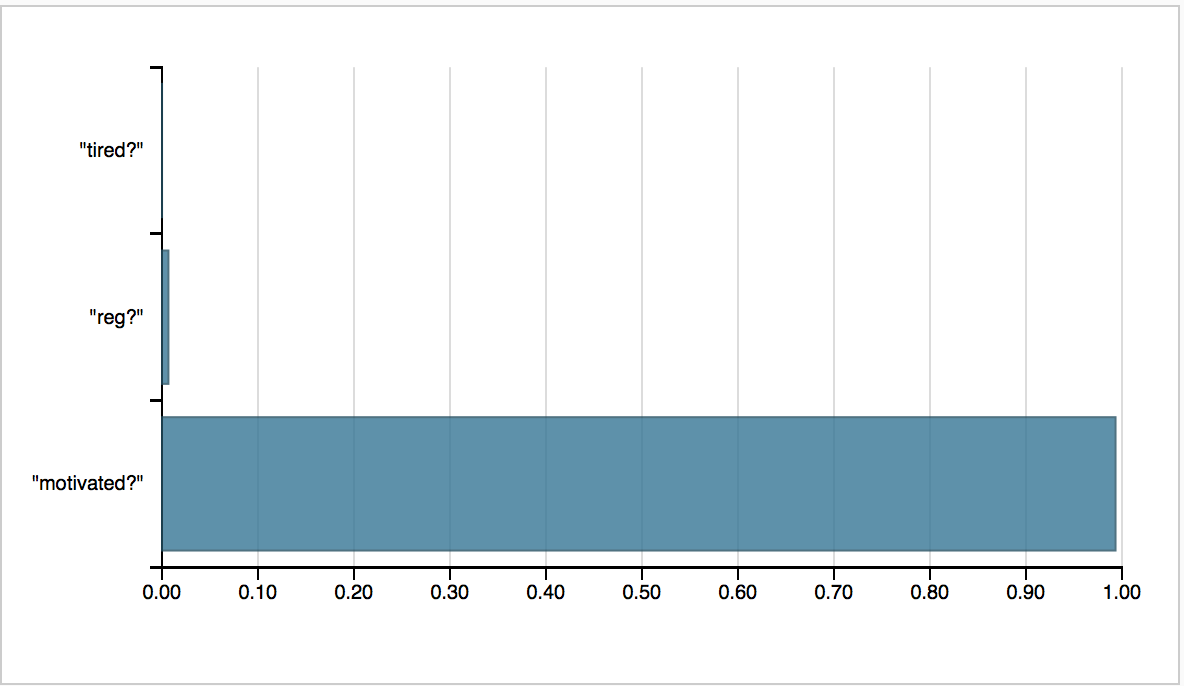
\includegraphics[scale=.71]{only_yes_dist.png}
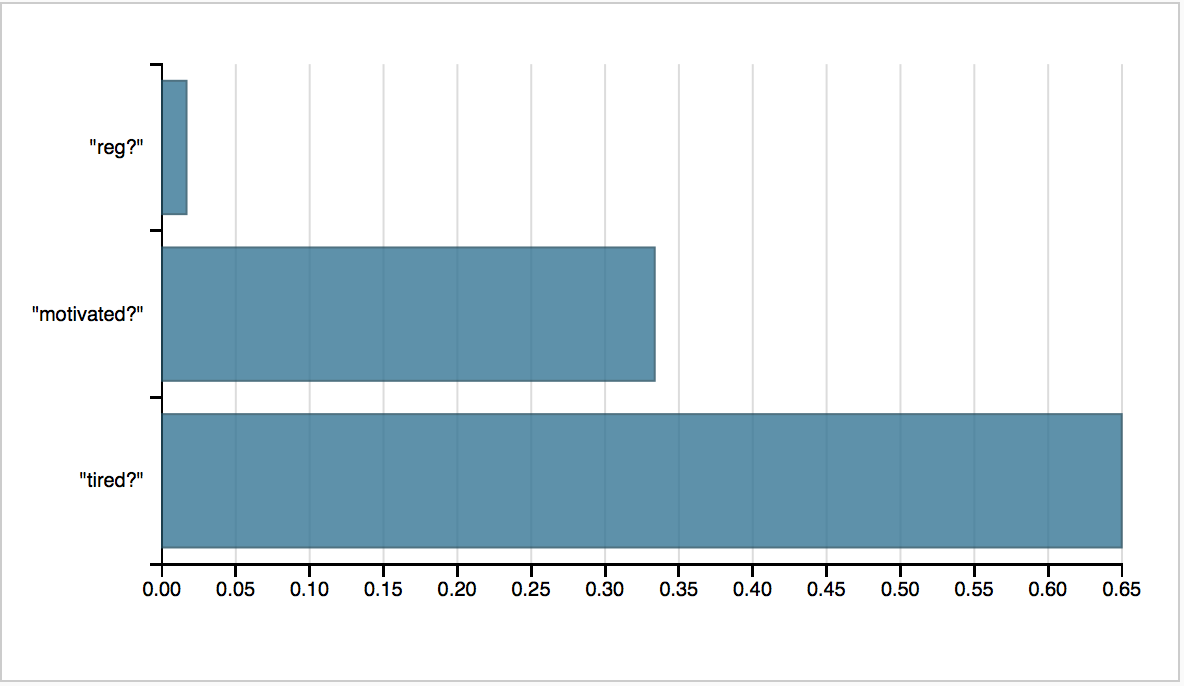
\includegraphics[scale=.71]{full_polar_dist.png}
\caption{The top panel displays the likelihood of Mary asking different questions given the standard literal listener who returns the distribution of worlds where the question is true. The bottom panel displays the same likelihoods given partition semantics that allow the literal listener to return the distribution of worlds where the answer is `no' when this is the appropriate cell of the partition. The bottom panel is closer to our intuition -- that the questioner is primarily concerned about stopping the belt when workers are not tired.}
\end{figure}

We now extend the model to allow for ``no" answers. This works by utilizing the standard Groenendijk partition semantics \cite{GroenendijkStokhof84_SemanticsOfQuestions}. Instead of returning a distribution over worlds in which the utterance is true, the literal answerer will return a distribution over worlds in the appropriate cell of the partition. If the answer to the question is true in the given world, the answerer will return that world, but if it is false, they will return a distribution over the remaining worlds that it could be. 

Formally, suppose we first fix a question utterance $u$. This question creates a partition $P_u$ on the space of possible worlds. For every world $w^*$ that could be the case (and the questioner does not know which is \emph{actually} the case), one cell of this partition is selected by the answerer, denoted $P_u(w^*)$, containing one or more possible worlds. We can then compute the expected value of the decision problem given $w^*$ to be 
$$\max_{a\in\mathcal{A}}\left[\sum_{w\in P_u(w^*)}P(w|P_u(w^*)) \times U(a, w)\right]$$
using a hard max rule over the set of actions. Note that the inner sum ranges over the worlds in the selected cell of the partition. The questioner then marginalizes over the possible values of $w^*$ to get the expected value of the question given utterance $u$. By picking the $u$ that maximizes this expected utility, we get a decision rule for optimally selecting questions.



%\begin{mylisting}
%var literalAnswerer = function(utt, w) {
%  Enumerate(function(){
%    var partition = span(function(b){return meaning(utt, b)}, [0,1,2])
%    var answer_set = (_.contains(partition[0], w) ? partition[0] :
%                      partition[1])
%    var i = randomInteger(answer_set.length);
%    return answer_set[i]
%  })
%}
%
%var valDP_hardMax = function(utt, dp) {
%  var res = maxWith(function(a){
%    expectation(Enumerate(function(){
%      var true_w = worldPrior()
%      var exp = expectation(Enumerate(function(){
%        var w = utt == "null" ? worldPrior() : sample(literalAnswerer(utt, true_w));
%        return dp(a, w);
%      }), function(v) {return v})
%      return true_w * exp;
%    }), function(v) {return v})
%  }, [0,1,2]);
%  return res[1];
%}
%
%print(questioner(dp_factory))
%\end{mylisting}

The distribution we get after running our model is shown in the bottom panel of Figure 1. We now recover the intuitive 'best question'. This is an encouraging result, demonstrating that the standard RSA model must be extended with partition semantics to qualitatively match our intuitions. Of course, whether this prediction is bourne out by humans is an empirical question. This task is similar to those used in recent work on interventions in causal systems and information foraging \cite[e.g.]{CoenenRehderGureckis14_InterveneCogSci} and could be interesting in its own right, but is not directly relevant to the questions at issue in this proposal. 

In order to derive predictions for hypothesis (1), where the answerer gives an over- or under-informative response, we must first introduce the ability to give non-polar responses. Considering a real situation in which a factory manager is asking a worker whether they were motivated, it would not be too unexpected if the worker responded, ``No, we're actually quite tired if you want to know." If the worker were always allowed to (overinformatively) state the true world in the current model, then their behavior would be trivial and the question wouldn't matter. To make the situation interesting, then, there must be some uncertainty over the decision problem that the questioner is facing (i.e. selected from some `dpPrior'). As far as hypothesis (2) is concerned, there's currently no reason for the questioner in the model to reason pragmatically about the answerer, since the answerer doesn't take the questioner into account in the first place.

The more complex issues we're concerned with in this proposal are easier to see in a more natural example using a taxonomy over a hierarchical domain. Suppose that there are four states of the world: the answerer can have a dalmatian ($d_1$), a poodle ($d_2$), a Persian cat ($c_1$), or a basil plant ($b_1$). Note that for either $d_1$ or $d_2$, it is also true that they have a dog $(d)$, and conversely if you know that they have a dog, this restricts the set of possible worlds to either $d_1$ or $d_2$. Note also that for either $d$ or $c_1$, it is also true that they have an animal $a$, which conversely restricts the set of possible worlds to $d_1, d_2,$ and $c_1$.  These relationships are visualized in Fig. \ref{tree}. 

\begin{figure}
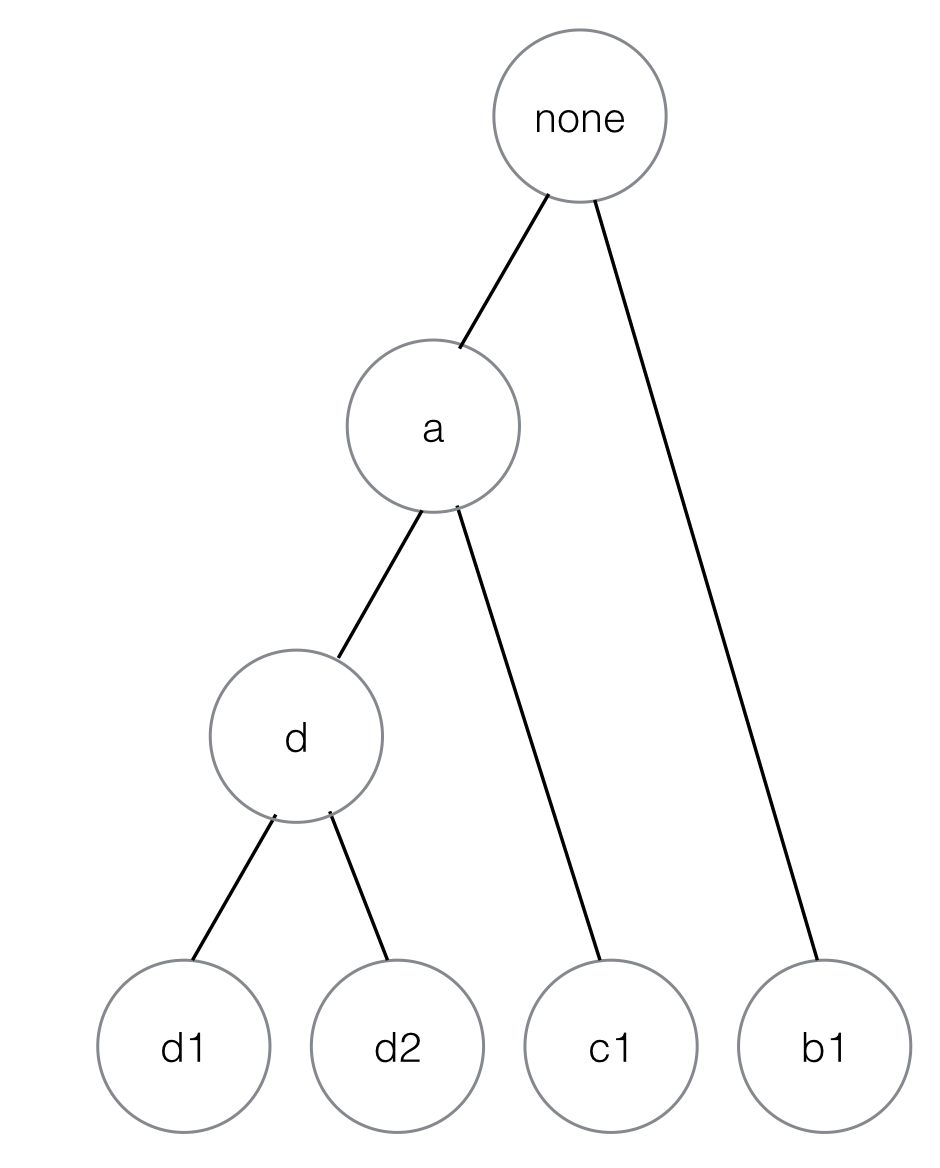
\includegraphics[scale=.5]{hierarchy.png}
\caption{Hierarchy of world states. Questioners can query at any point in the hierarchy, inducing different partitions over the leaves. For example, asking ``do you have a dog ($d$)?'' creates the partition $\langle (d_1, d_2), (c_1, b_1)\rangle$}
\label{tree}
\end{figure}

The next step is to generalize our model to allow for the questioner to make a query at any point in the hierarchy of questions, so in addition to asking questions about the leaves like ``do you have a dalmatian?'' or ``do you have a basil plant?'' , the agent can ask ``do you have an dog?'' This would maximize the value of the decision problem, for instance, in the case that the same action is preferred for states $d_1$ and $d_2$, but a different action is preferred for the other states. Thus, we can formulate different decision problems by changing the utilities over states. Once this is working, we can create a pragmatic answerer that reasons about the decision problem the questioner is trying to solve, conditioning on the utterance the questioner makes. It may turn out that they need to know something about the scenario as well. Unlike the factory problem, telling the questioner the direct state of the world is not the best answer for every decision problem. These steps will open up new questions about the appropriate partition semantics, and suggest new experiment conditions to run.

\section{Experiments}

There is a good precedent for empirically studying the over- and under-informative responses relevant to our first hypothesis \cite{Clark79_IndirectSpeechActs, GibbsBryant08_OptimalRelevance}, although  less precedent for studying the choice of questions and the extent to which the questioner must reason about the answerer's mental state. We will first discuss some pilot work clarifying the kinds of inferences people make about intentions behind questions and answers. This work established a stimulus set of hierarchical domains, allowing for over- and under-informative responses that can serve as a target case for our model. Finally, it revealed some interesting implicatures in this hierarchical domain, which appear to be moderated by the perceived intentions of the speaker. Following these observations, we propose a follow-up experiment to directly manipulate perceived intentions and measure their effect on answer appropriateness.

\textbf{Experiment 1}. Our pilot experiment  elicited explanations of questions and answers, allowing us to get some intuitions for the kinds of inferences being made. Participants saw a question of the form ``Do you have a $x$?'', with $x$ being drawn from four domains: pets ($x=$`dog'), vehicles ($x=$`car'), clothes ($x=$`shirt'), and food ($x=$`Mexican food'). They were asked why someone might be asking this question. Next, an answer was displayed at one of four relations to the class of $x$: the subset (e.g. `dalmatian'), the identity (e.g. `dog'), the superset (e.g. `animal'), and the sibling (e.g. `cat'). Participants were asked why someone might give this answer. Finally, they were shown a slider and asked to rate how helpful this answer is with respect to the earlier question. Each participant saw four question-answer pairs: one of each domain and one of each answer type, randomly paired. 

We informally tagged the question explanations into three classes: polite requests for the answerer to do something, requests for information, and conversation. The car, shirt, and food questions were overwhelmingly interpreted as polite requests. This reflects a strong prior over what objects are commonly borrowed -- in the absence of any additional context, someone probably wants a ride if they ask you whether you have a car. However, the `dog' domain does not admit the polite request interpretation as easily; it is rare for one person to borrow another person's dog. Instead, responses were divided evenly between `information' and `conversation' intentions. For an example of the information inference, one participant supposed that the questioner is allergic to dogs and wants to know whether their friend has one before coming over for dinner. 

These differences in inferred intentions suggest that it's not appropriate to collapse across domains in looking at the helpfulness of different answer relations. If you want a ride, then the superset answer ``I have a vehicle'' is still quite helpful, whereas if you are looking for information concerning your dog allergy, the superset answer ``I have an animal'' is not helpful at all. Experiment 2 is designed to address this by explicitly manipulating the decision problem at stake.

Finally, it is worth noticing the various implicatures that participants drew from answer utterances. For example, if the questioner asks ``Do you have a dog?'' and the answerer replies ``I have a cat,'' the sibling relation, participants commonly explained the answer as implying that they did \emph{not} have a dog. This is a result of literal semantics given the assumption that having a cat and a dog is mutually exclusive (i.e. that the answerer only has one pet). More curiously, though, the superset relation was also commonly given a ``no, but'' interpretation, despite being consistent with both a 'yes' and 'no' reading. This can be understood pragmatically: if they had a dog, they would have said so. Therefore their vagueness implies that they don't have a dog. This is something we would like to see emerge from our model, eventually.

\textbf{Experiment 2} Recall that we found three primary classes of intentions in the previous experiment: polite requests, information queries, and indefinite conversation. We hypothesize that these intentions roughly correspond with different decision problems, and that different decision problems admit different answers as appropriate. To test how the appropriateness of answers varies systematically with intention, and also to probe the effect of intention on pragmatic implicature, we explicitly present participants with scenarios inducing different preferred intentions. Here are three examples in the dog domain. 

\begin{quote}
\begin{enumerate} [1.]
\item You're at a party making polite conversation. Susan asks ``Do you have a dog?'' You respond $x$.
	\begin{enumerate}[(a)]
     \item How appropriate is this answer?
     \item To what extent does this answer imply that you have a dog?
	\end{enumerate}
\item You know Susan's family is coming into town and she wants to amuse them with an adorable pet. Susan calls you and asks ``Do you have a dog?'' You respond $x$.
     \begin{enumerate}[(a)]
     \item How appropriate is this answer?
     \item To what extent does this answer imply that you have a dog?
     \end{enumerate}

\item Susan is visiting your house for dinner, and you know she is allergic to dogs. Before coming over, Susan asks, ``Do you have a dog?'' You respond $x$.
     \begin{enumerate}[(a)] 
     \item How appropriate is this answer?
     \item To what extent does this answer imply that you have a dog?
     \end{enumerate}
\end{enumerate}
\end{quote}

The results of this experiment could help us formulate utilities for different decision problems in our model. In the `conversation' case, we predict that only subset and sibling answers would be regarded as appropriate, since utility is placed on offering further detail. In the `polite request' case, any of the four responses should work, since Susan just needs some pet and it doesn't matter which. In the `information' case, only the identity (and perhaps the subset) would be considered appropriate. Once we construct the model (or multiple models) described in the previous section, further experiments will be necessary to test their predictions.

\section{Discussion}

We conclude by discussing some further issues raised by the approach laid out above. One curiosity is the apparent lack of an explicit QUD (question under discussion) in our problem formulation. It remains implicit in the way the literal answerer partitions the space of answers (where the QUD is assumed to be identical to the uttered question), but an alternative formulation of the problem would have answerers inferring intentions via a space of \emph{QUD}s rather than via decision problems. It may turn out that these two formulations are equivalent: that every QUD induces a set of utilities forming a decision problem, and every decision problem favors a corresponding QUD. This is not obvious, however, and it may turn out that one formulation is more general than the other. 

There is some connection between the Q\&A phenomena discussed in this proposal and the problem of basic-level reference discovered by Elinor Rosch \cite{RoschMervisGray___BoyesBraem76_BasicObjects}. She noted that there is an intermediate level of specificity preferred by speakers in the absence of other cues: if a speaker wanted to point out a German sheepdog in your backyard, they would be more likely to say `look, there's a dog' rather than `look, there's an animal', or `look, there's a German sheepdog.' Her explanation for the phenomenon was a joint optimization of two psychological forces: (1) cognitive economy, which places a cost on dividing the world into two many separate categories and (2) cue validity, which prefers a set of categories that are maximally differentiated from one another in terms of their features. Momentarily setting aside the argument from non-linguistic tasks, our approach might suggest a more communicative explanation for basic-level reference. In the same way that answerers in our model gravitate toward the level of specificity required by their inference about the questioner's intentions, speakers in a reference-generation task may gravitate toward labels that are most informative with respect to the listener's goals. These predictions could be fit into our Q\&A approach as the answer to an implicit question like ``what is that?'' This communicative account predicts that speakers might systematically deviate from basic-level predictions given some context about the mental state of the listener. If you know your friend is a dog enthusiast, for example, then a more specific level of reference is preferable. 

Finally, it's fun to brainstorm potential applications of a successful theory of Q\&A behavior for the larger world of social science. Politicians are often accused of giving non-informative answers to reporters and audience members\cite{Bull94_QuestionsRepliesNonRepliesPoliticalInterviews}, kids ask better questions during tutoring interactions than classroom interactions \cite{GraesserPerson94_QuestionAskingTutoring}, talk show hosts rely on  question formats with lightly concealed intentions to drive arguments with their guests \cite{Ilie99_Q_and_A_TalkShows}, and different questions are chosen during cross-examination if the witness is regarded as hostile or non-cooperative  \cite{Wellman97_CrossExamination}. It could be useful to study some of these non-standard Q\&A domains to clarify how typical conversation participants behave.  One plausible collaboration with computational linguists would be to train a classifier on a court transcript corpus to distinguish between direct examination utterance and cross-examination utterance. This could pinpoint the features that are common to `helpful' replies, and the differences in questions when directed at cooperative vs. non-cooperative answerers. It's telling that exceptions to the `no leading questions' rule are only allowed during the cross-examination phase. Overall, it's clear that the Q\&A domain raises many important and fascinating research questions, though Nature is not necessarily an informative answerer. The computational and experimental steps outlined in this proposal are directed at the most coherent and tractable of these questions, and the dialogue will continue.

\bibliography{fyp_refs}

\bibliographystyle{ieeetr}


\end{document}  
